\section{Grafik Türleri}
Veri bilimi, karmaşık veri setlerinden anlamlı bilgiler çıkarmak için çeşitli teknikler ve araçlar kullanır. Bu tekniklerden biri de grafiklerdir. Grafikler, verileri görsel olarak temsil ederek, desenleri ortaya çıkarır, ilişkileri gösterir ve bilgileri daha anlaşılır hale getirir.

\begin{figure}[h]
    \centering
    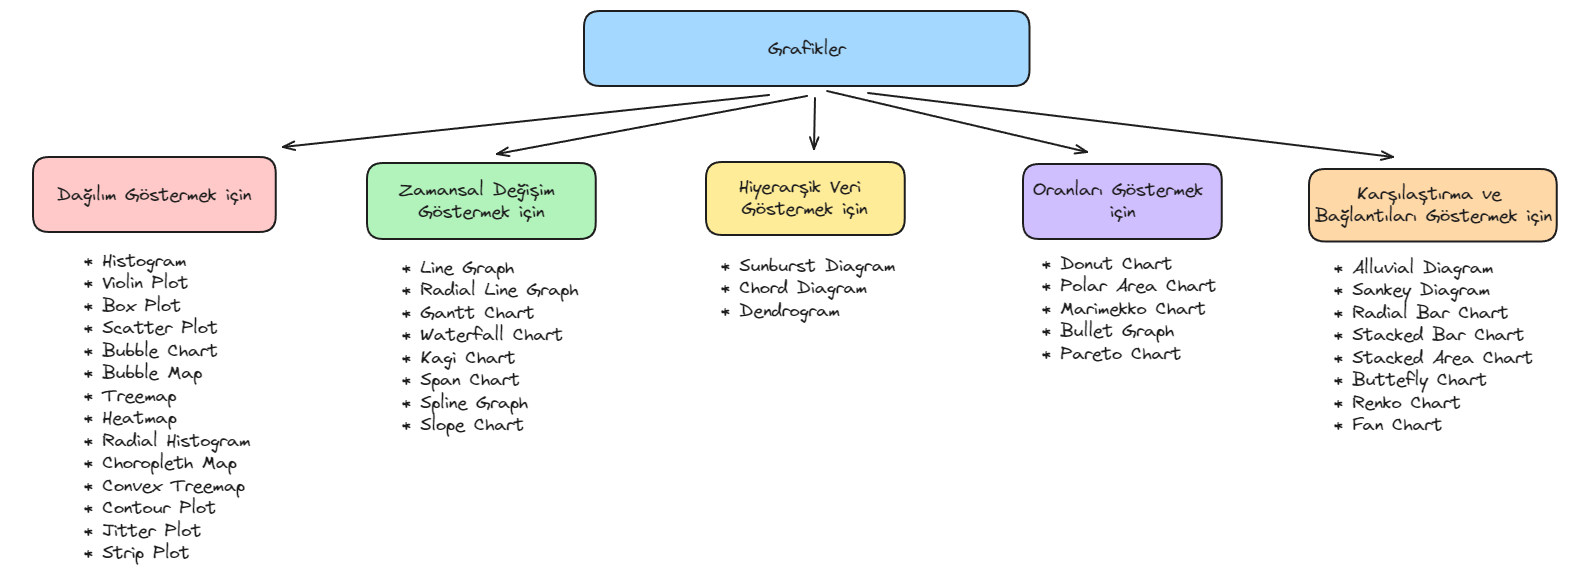
\includegraphics[width=1\textwidth]{images/graph_types.png}
    \caption{Grafik türleri.}
    \label{fig:enter-label}
\end{figure}

\newpage

\subsection{Alluvial Diagram}
Zamanla değişen kategorik değişkenler arasındaki ilişkileri göstermek için tercih edilirler. Değişkenler paralel olarak dikey eksene atanır. Değerler her eksende bloklarla gösterilir. Blok yüksekliği küme boyutunu, aradaki bağlantı yolu ise her iki blokta yer alan bileşenlerin boyutunu gösterir.

\begin{lstlisting}[language=Python]
import plotly.graph_objects as go

fig = go.Figure(data=[go.Sankey(
    node = dict(
      pad = 10,
      thickness = 25,
      line = dict(color = "black", width = 0.2),
      label = ["Satis", "Muhendislik", "Pazarlama"],
      color = "blue"
    ),
    link = dict(
      source = [2020, 2021, 2022],
      target = [1, 2, 3],
      value = [100, 120, 150],
  ))])

fig.update_layout(title_text="Sankey Diagram", font_size=10)
fig.show()
\end{lstlisting}

\begin{figure}[h]
    \centering
    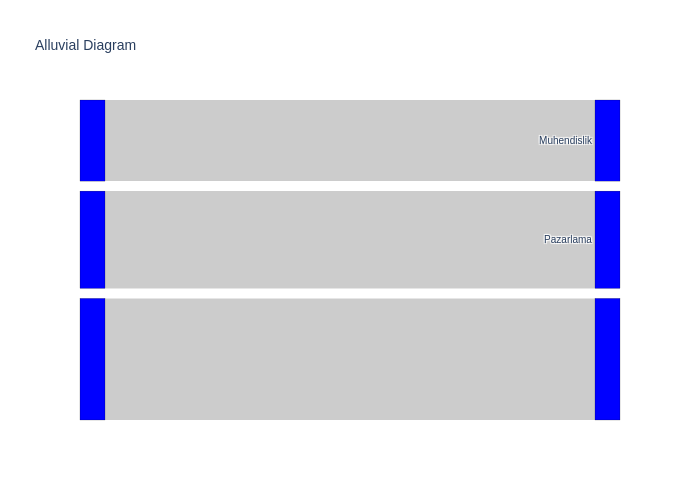
\includegraphics[width=0.8\textwidth]{images/alluvial_diagram.png}
    \caption{Alluvial diagram örneği.}
    \label{fig:enter-label}
\end{figure}

\newpage

\subsection{Sankey Diagram}
Akışları, ilişkileri ve kitleleri göstermek için kullanılır. Örneğin enerji akışları, bütçe dağılımları, materyal akışları, proses ilişkileri, kaynak dağılımı, bir sistemdeki akışlar vb. Okların kalınlığı akış miktarın, işlemler arasındaki ilişkiyi veya kaynakların dağılımı gösterir. Okların yönü, akışın hangi yönde olduğunu gösterir.

\begin{lstlisting}[language=Python]
import matplotlib.pyplot as plt
from matplotlib.sankey import Sankey

flows = [120, 80, 200, -180, -30, -70, -50]
labels = ['Giris', 'Islem 1', 'Islem 2', 'Islem 3', 'Islem 4', 'Islem 5', 'Cikis']

sankey = Sankey()
sankey.add(flows=flows, labels=labels, orientations=[0, 1, 1, -1, -1, -1, 0])
sankey.finish()

plt.title('Ornek Sankey Diagram')
plt.show()
\end{lstlisting}

\begin{figure}[h]
    \centering
    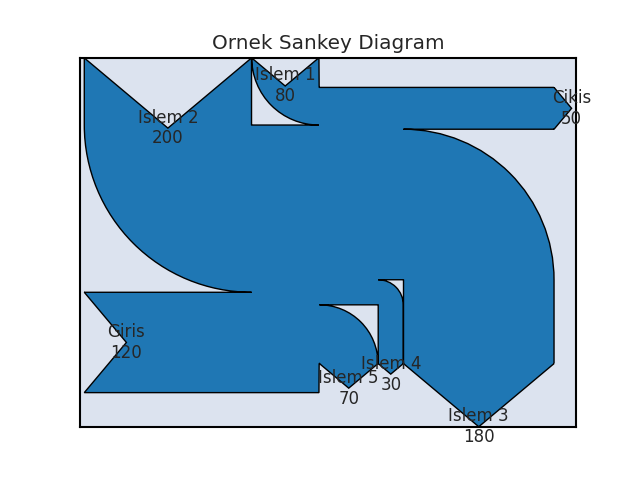
\includegraphics[width=0.7\textwidth]{images/sankey_diagram.png}
    \caption{Sankey diagram örneği.}
    \label{fig:enter-label}
\end{figure}

\newpage

\subsection{Donut Chart}
Pie chart'a benzer fakat ortası boştur. Kategorik bir bütünün parçalarının oransal dağılımını gösterir. Dilimi büyük olanın oransal dağılımı fazladır.

\begin{lstlisting}[language=Python]
import matplotlib.pyplot as plt

labels = ['A', 'B', 'C', 'D']
sizes = [25, 30, 20, 25]

fig, ax = plt.subplots()
ax.pie(sizes, labels=labels, autopct='%1.1f%%', startangle=90, wedgeprops=dict(width=0.3))
ax.axis('equal')

plt.title('Ornek Donut Chart')
plt.show()
\end{lstlisting}

\begin{figure}[h]
    \centering
    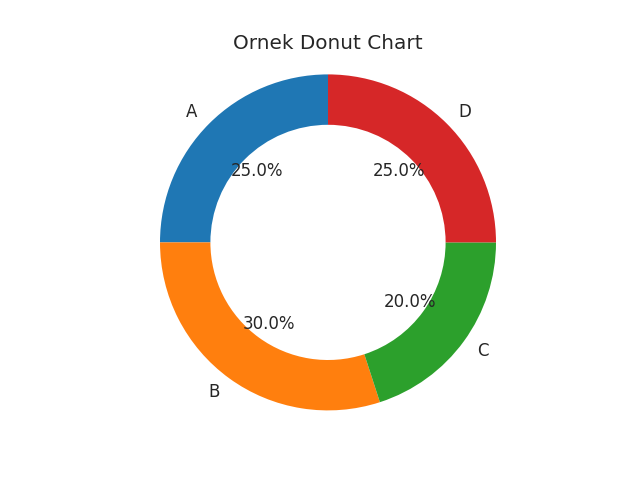
\includegraphics[width=0.7\textwidth]{images/donut_chart.png}
    \caption{Donut chart örneği.}
    \label{fig:enter-label}
\end{figure}

\newpage

\subsection{Line Graph}
Sürekli bir değişkenin belirli aralıklarla ölçülen veya zamanla değişen değerlerini göstermek için kullanılır.

\begin{lstlisting}[language=Python]
import matplotlib.pyplot as plt

x = [1, 2, 3, 4, 5]
y = [10, 15, 13, 18, 20]

plt.plot(x, y, marker='o', linestyle='-')

plt.title('Ornek Line Graph')
plt.xlabel('X Ekseni')
plt.ylabel('Y Ekseni')
plt.grid(True)
plt.show()

\end{lstlisting}

\begin{figure}[h]
    \centering
    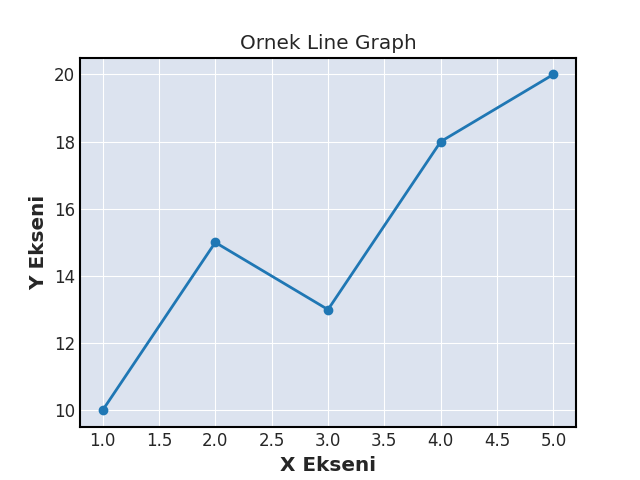
\includegraphics[width=0.7\textwidth]{images/line_graph.png}
    \caption{Line graph örneği.}
    \label{fig:enter-label}
\end{figure}

\newpage

\subsection{Radial Bar Chart}
Birbirine bağlı veya ilişkili kategorik verileri karşılaştırmak için kullanılır.

\begin{lstlisting}[language=Python]
import matplotlib.pyplot as plt
import numpy as np

categories = ['A', 'B', 'C', 'D']
values = [20, 35, 30, 25]

angles = np.linspace(0, 2 * np.pi, len(categories), endpoint=False).tolist()

fig, ax = plt.subplots(figsize=(6, 6), subplot_kw=dict(polar=True))
bars = ax.bar(angles, values, width=0.5, color='skyblue', edgecolor='black')

ax.set_xticks(angles)
ax.set_xticklabels(categories)

plt.title('Ornek Radial Bar Chart')
plt.show()
\end{lstlisting}

\begin{figure}[h]
    \centering
    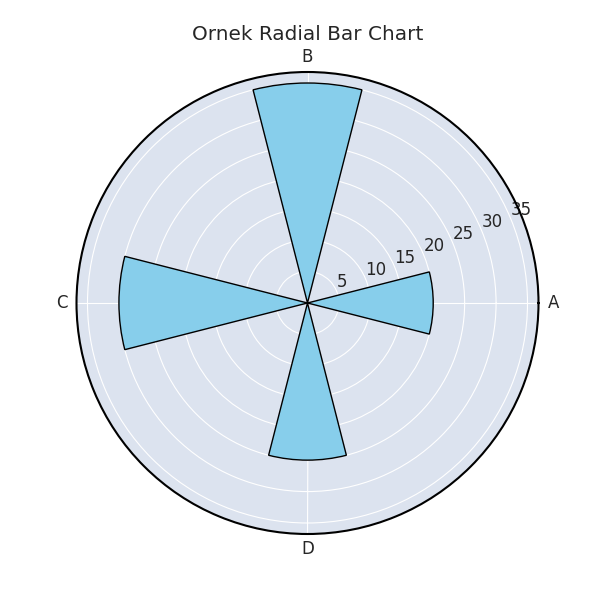
\includegraphics[width=0.7\textwidth]{images/radial_bar_chart.png}
    \caption{Radial bar chart örneği.}
    \label{fig:enter-label}
\end{figure}

\newpage

\subsection{Polar Area Chart}
Verilerin oransal dağılımını göstermek için kullanılır.

\begin{lstlisting}[language=Python]
import matplotlib.pyplot as plt

categories = ['A', 'B', 'C', 'D']
values = [20, 35, 30, 25]

fig, ax = plt.subplots(figsize=(6, 6), subplot_kw=dict(polar=True))
bars = ax.bar(categories, values, width=0.5, color='skyblue')

plt.title('Ornek Polar Area Chart')
plt.show()
\end{lstlisting}

\begin{figure}[h]
    \centering
    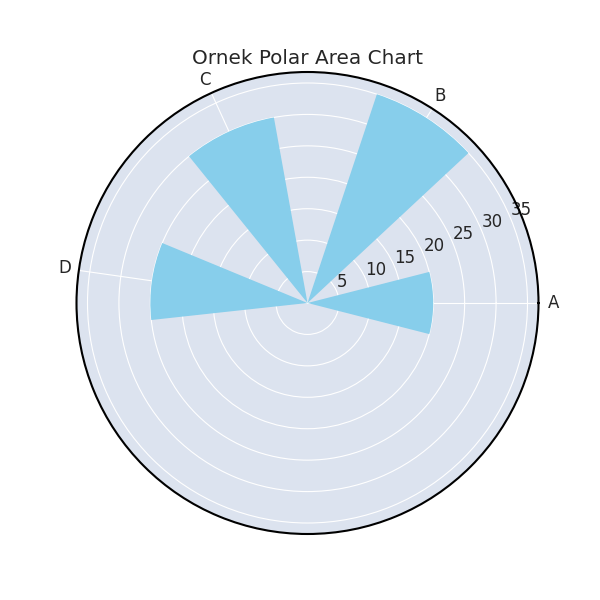
\includegraphics[width=0.7\textwidth]{images/polar_area_chart.png}
    \caption{Polar area örneği.}
    \label{fig:enter-label}
\end{figure}

\newpage

\subsection{Bar Chart}
Kategorik verilerin sayısal değerlerini göstermek için kullanılır.

\begin{lstlisting}[language=Python]
import matplotlib.pyplot as plt

categories = ['A', 'B', 'C', 'D']
values = [20, 35, 30, 25]

plt.figure(figsize=(8, 6))
plt.bar(categories, values, color='skyblue')

plt.title('Ornek Bar Chart')
plt.xlabel('Kategoriler')
plt.ylabel('Degerler')
plt.show()
\end{lstlisting}

\begin{figure}[h]
    \centering
    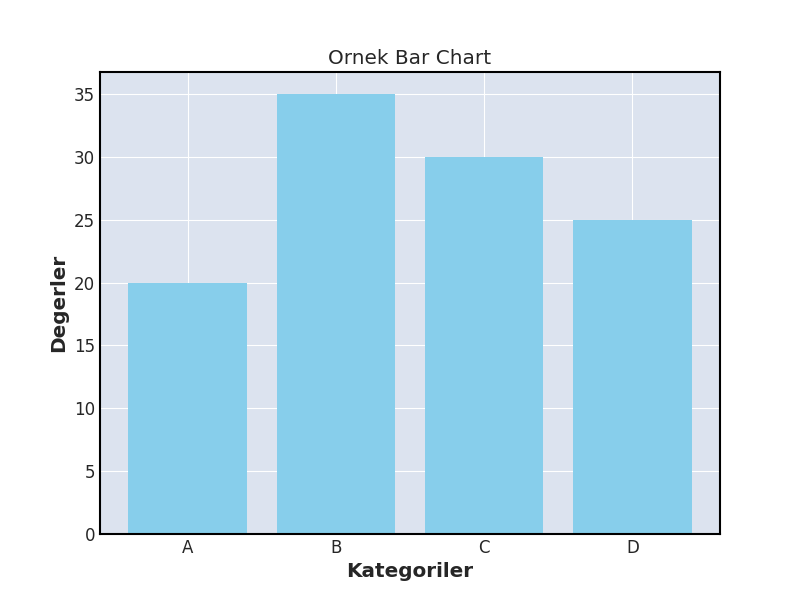
\includegraphics[width=0.7\textwidth]{images/bar_chart.png}
    \caption{Bar chart örneği.}
    \label{fig:enter-label}
\end{figure}

\newpage

\subsection{Radial Histogram}
Özellikle dairesel veya halka şeklindeki veri yapısını vurgulamak ve veri setinin yoğunluk veya dağılımını görsel olarak göstermek için kullanılır.

\begin{lstlisting}[language=Python]
import matplotlib.pyplot as plt
import numpy as np

np.random.seed(0)
r = np.random.normal(0, 1, 1000)
theta = 2 * np.pi * np.random.rand(1000)

plt.figure(figsize=(6, 6))
plt.hist(theta, bins=30, color='skyblue')

plt.title('Ornek Radial Histogram')
plt.show()
\end{lstlisting}

\begin{figure}[h]
    \centering
    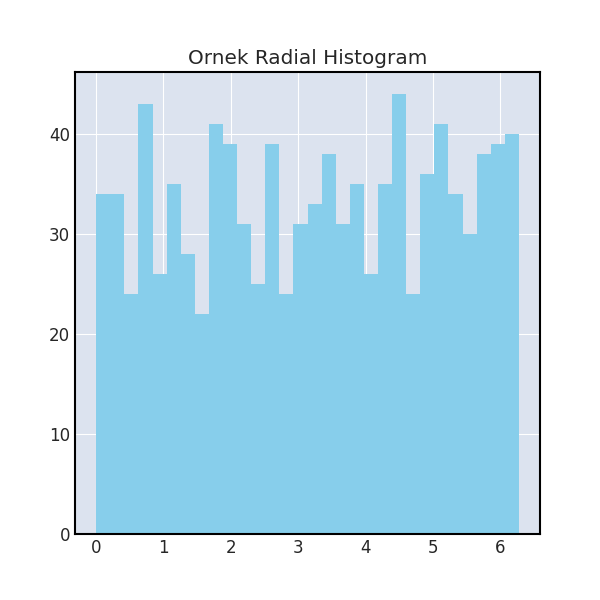
\includegraphics[width=0.7\textwidth]{images/radial_histogram.png}
    \caption{Radial histogram örneği.}
    \label{fig:enter-label}
\end{figure}

\newpage

\subsection{Sunburst Diagram}
Bir bütün parçalarını ve parçaların hiyerarşik yapılarını göstermek için kullanılır. Kategorik verilerin alt kategorilerle ilişkisini ve her bir kategorinin toplam içindeki oransal büyüklüğünü vurgulamak için tercih edilir.

\begin{lstlisting}[language=Python]
import plotly.graph_objects as go

fig = go.Figure(go.Sunburst(
    labels=["A", "B", "C", "D", "E", "F"],
    parents=["", "A", "B", "B", "C", "C"],
    values=[10, 15, 8, 7, 12, 5],
))

fig.update_layout(title='Ornek Sunburst Diagram')
fig.show()
\end{lstlisting}

\begin{figure}[h]
    \centering
    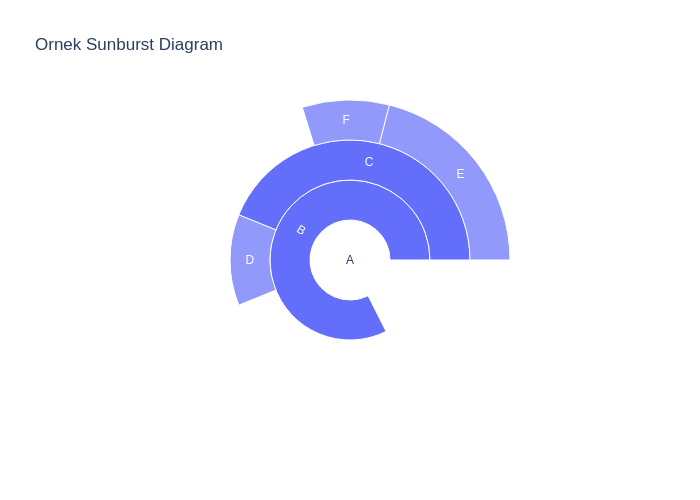
\includegraphics[width=0.7\textwidth]{images/sunburst_diagram.png}
    \caption{Sunburst diagram örneği.}
    \label{fig:enter-label}
\end{figure}

\newpage

\subsection{Treemap}
Hiyerarşik verileri dikdörtgen kutuların alanları olarak görselleştiren bir grafik türüdür. Bir bütünün parçalarını ve parçaların hiyerarşik yapılarını göstermek için kullanılır.

\begin{lstlisting}[language=Python]
import matplotlib.pyplot as plt
import squarify

sizes = [25, 30, 20, 15, 10]

squarify.plot(sizes=sizes, label=["A", "B", "C", "D", "E"], alpha=0.7)

plt.title('Ornek Treemap')
plt.axis('off')
plt.show()
\end{lstlisting}

\begin{figure}[h]
    \centering
    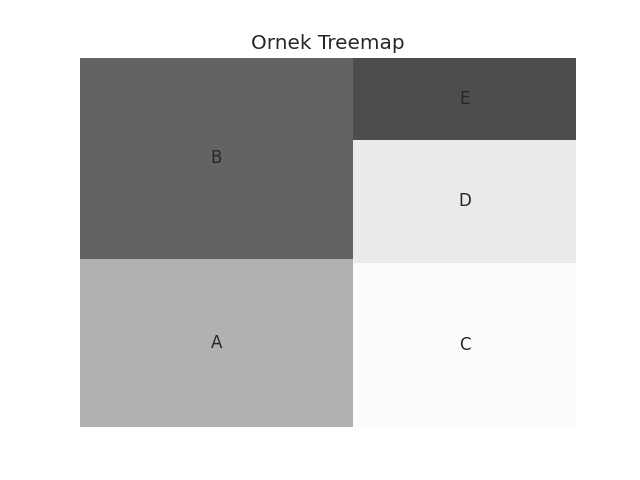
\includegraphics[width=0.7\textwidth]{images/treemap.png}
    \caption{Treemap örneği.}
    \label{fig:enter-label}
\end{figure}

\newpage

\subsection{Heatmap}
Sayısal verilerin yoğunluğu veya ilişkilerini renklerle göstermek için kullanılır. Her bir hücre, veri setindeki bir iki değişken arasındaki ilişki değerini temsil eder.

\begin{lstlisting}[language=Python]
import seaborn as sns
import numpy as np

data = np.random.rand(10, 10)

sns.heatmap(data, cmap='YlGnBu')

plt.title('Ornek Heatmap')
plt.show()
\end{lstlisting}

\begin{figure}[h]
    \centering
    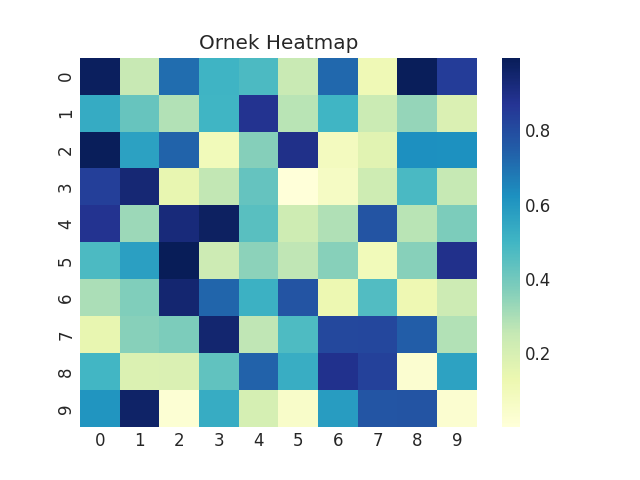
\includegraphics[width=0.7\textwidth]{images/heatmap.png}
    \caption{Heatmap örneği.}
    \label{fig:enter-label}
\end{figure}

\newpage

\subsection{Stacked Bar Chart}
Kategorik verilerin karşılaştırılması için kullanılır. Farklı kategoriler içindeki alt kategorilerin değerlerini karşılaştırmak için kullanılır.

\begin{lstlisting}[language=Python]
import matplotlib.pyplot as plt

categories = ['A', 'B', 'C', 'D']
values1 = [20, 35, 30, 25]
values2 = [15, 25, 20, 15]

plt.figure(figsize=(8, 6))
plt.bar(categories, values1, color='skyblue', label='Grup 1')
plt.bar(categories, values2, bottom=values1, color='orange', label='Grup 2')

plt.title('Ornek Stacked Bar Chart')
plt.xlabel('Kategoriler')
plt.ylabel('Degerler')
plt.legend()
plt.show()
\end{lstlisting}

\begin{figure}[h]
    \centering
    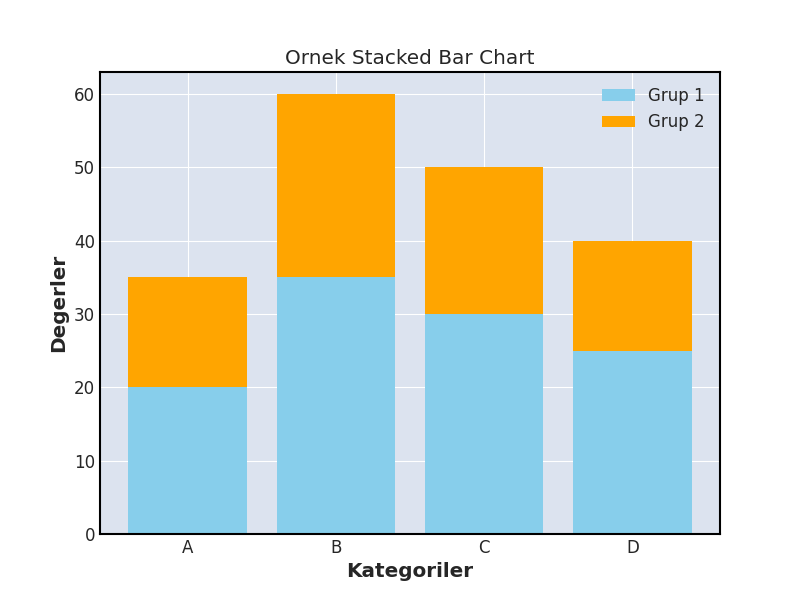
\includegraphics[width=0.7\textwidth]{images/stacked_bar_chart.png}
    \caption{Stacked bar chart örneği.}
    \label{fig:enter-label}
\end{figure}

\newpage

\subsection{Chord Diagram}
İlişkisel verileri ve bu veriler arasındaki bağlantıları daire içindeki yaylarla gösterir.

\begin{lstlisting}[language=Python]
import matplotlib.pyplot as plt
from matplotlib.sankey import Sankey

links = {
    ("A", "B"): 20,
    ("A", "C"): 15,
    ("B", "C"): 25,
    ("B", "D"): 10,
    ("C", "D"): 30
}

fig, ax = plt.subplots(figsize=(8, 8))
sankey = Sankey(ax=ax)
for link, weight in links.items():
    sankey.add(flows=[weight, -weight], labels=list(link))
sankey.finish()

plt.title('Ornek Chord Diagram')
plt.show() 
\end{lstlisting}

\begin{figure}[h]
    \centering
    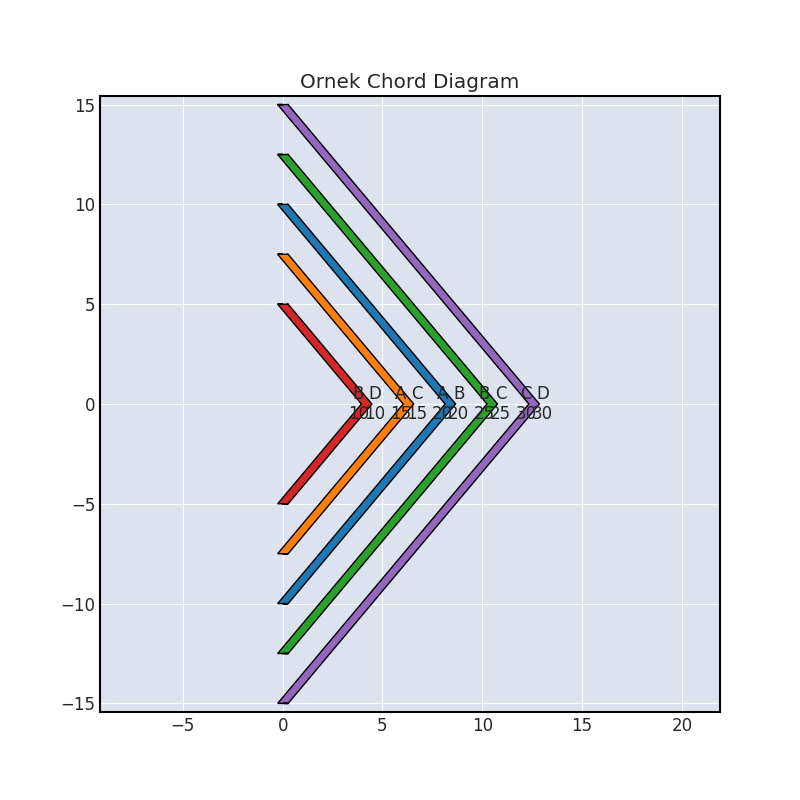
\includegraphics[width=0.6\textwidth]{images/chord_diagram.png}
    \caption{Chord diagram örneği.}
    \label{fig:enter-label}
\end{figure}

\newpage

\subsection{Choropleth Map}
Belirli bir coğrafi alandaki veri desenlerini, dağılımları veya farklılıkları görsel olarak anlamak için kullanılır.

\begin{lstlisting}[language=Python]
import geopandas as gpd
import random
import matplotlib.pyplot as plt

world = gpd.read_file(gpd.datasets.get_path('naturalearth_lowres'))

data = {country: random.randint(1, 10) for country in world['name']}
world['data'] = world['name'].map(data)

world.plot(column='data', cmap='YlOrRd', legend=True, figsize=(15, 10))
plt.title('Ornek Choropleth Harita')
plt.show() 
\end{lstlisting}

\begin{figure}[h]
    \centering
    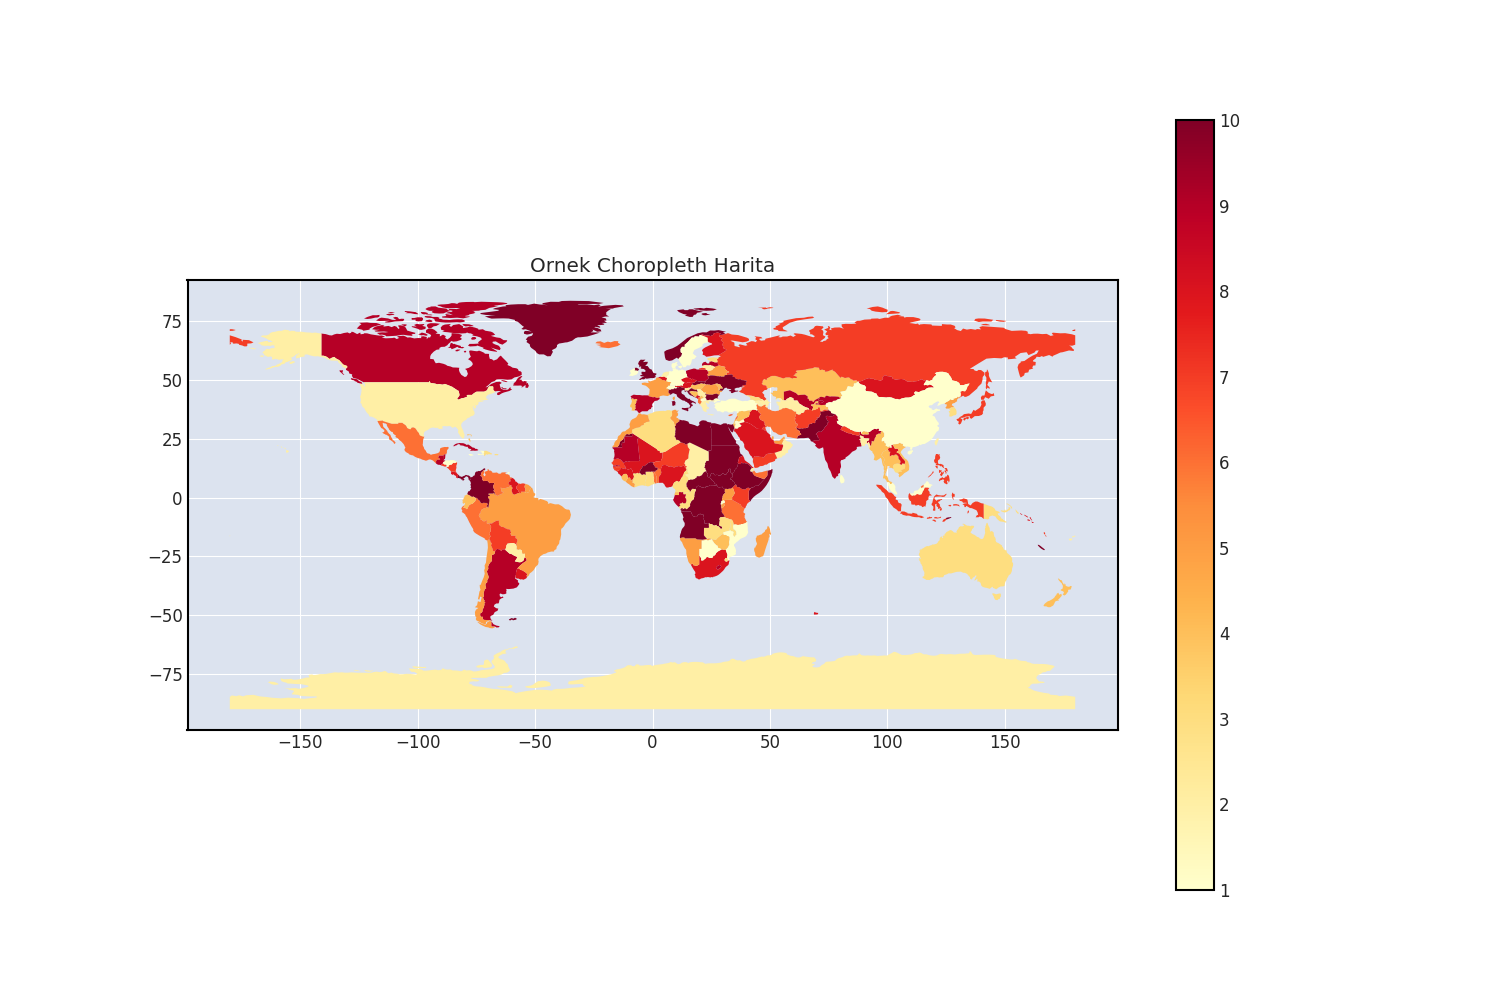
\includegraphics[width=0.7\textwidth]{images/choropleth_map.png}
    \caption{Choropleth map örneği.}
    \label{fig:enter-label}
\end{figure}

\newpage

\subsection{Radial Line Graph}
Genellikle zaman içinde değişen veya belirli bir dönemde farklı bir kategoriler arasındaki ilişkiyi göstermek için kullanılır. Her bir çizgi, bir kategori veya değişkeni, çizgilerin uzunlukları veri değerlerini temsil eder.

\begin{lstlisting}[language=Python]
import matplotlib.pyplot as plt
import numpy as np

categories = ['A', 'B', 'C', 'D']
values = [10, 20, 15, 25]

fig, ax = plt.subplots(subplot_kw=dict(polar=True))

theta = np.linspace(0, 2 * np.pi, len(categories), endpoint=False)
values += values[:1]
theta += theta[:1]

ax.plot(theta, values, marker='o')

ax.set_theta_offset(np.pi / 2)
ax.set_theta_direction(-1)

plt.title('Ornek Radial Line Graph')
plt.show()
\end{lstlisting}

\begin{figure}[h]
    \centering
    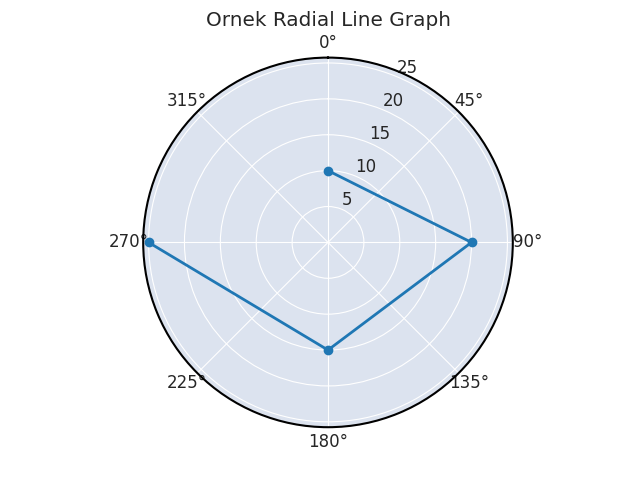
\includegraphics[width=0.7\textwidth]{images/radial_line_graph.png}
    \caption{Radial line örneği.}
    \label{fig:enter-label}
\end{figure}

\newpage

\subsection{Bubble Map}
Coğrafi bölgelerin veya noktaların harita üzerinde farklı büyüklükte veya renklerde dairelerle temsil edildiği bir harita türüdür.

\begin{lstlisting}[language=Python]
import plotly.express as px

data = dict(
    lat=[40.7128, 34.0522, 41.8781],
    lon=[-74.0060, -118.2437, -87.6298],
    text=['New York', 'Los Angeles', 'Chicago'],
    size=[20, 50, 30],
    color=[10, 20, 30]
)

fig = px.scatter_geo(data, lat='lat', lon='lon', text='text', size='size', color='color')
fig.update_geos(projection_type="natural earth")

fig.update_layout(title='Ornek Bubble Map')
fig.show()
\end{lstlisting}

\begin{figure}[h]
    \centering
    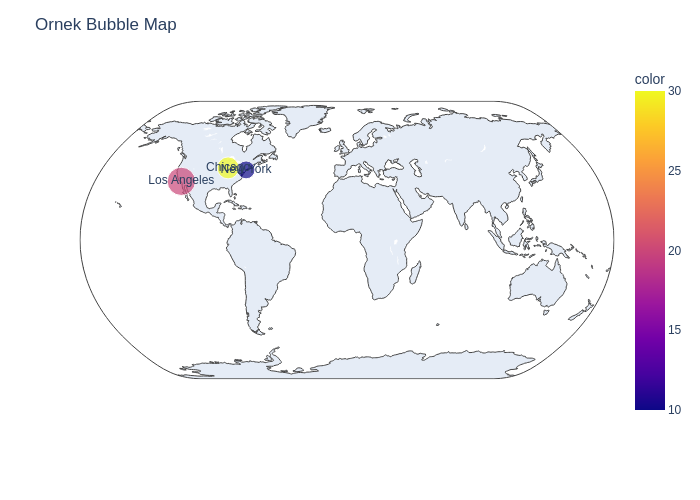
\includegraphics[width=0.7\textwidth]{images/bubble_map.png}
    \caption{Bubble map örneği.}
    \label{fig:enter-label}
\end{figure}

\newpage

\subsection{Bubble Chart}
İki değişken arasındaki ilişkiyi gösteren bir scatter plot ile birlikte üçüncü bir değişkenin büyüklüğünü veya yoğunluğunu da gösterir. Her bir nokta bir veri noktasını temsil ederken, noktanın büyüklüğü veya renk tonu üçünü değişkeni gösterir.

\begin{lstlisting}[language=Python]
import matplotlib.pyplot as plt

x = [1, 2, 3, 4, 5]
y = [10, 15, 20, 25, 30]
sizes = [40, 80, 120, 160, 200]

plt.scatter(x, y, s=sizes, alpha=0.5)

plt.title('Ornek Bubble Chart')
plt.xlabel('X Degiskeni')
plt.ylabel('Y Degiskeni')
plt.show()
\end{lstlisting}

\begin{figure}[h]
    \centering
    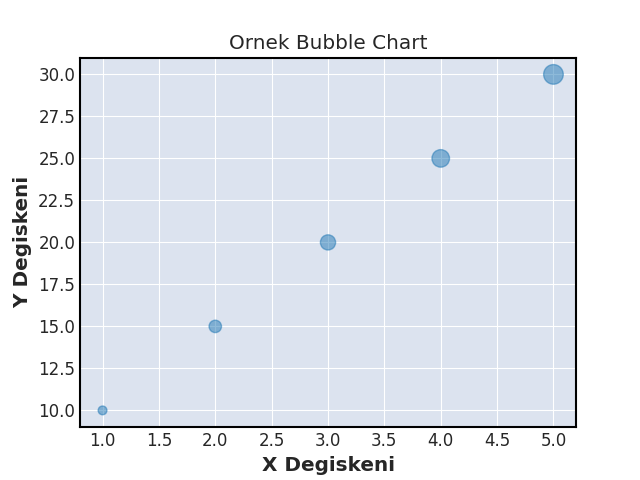
\includegraphics[width=0.7\textwidth]{images/bubble_chart.png}
    \caption{Bubble chart örneği.}
    \label{fig:enter-label}
\end{figure}

\newpage

\subsection{Violin Plot}
Box plot dağılım özelliklerini daha ayrıntılı bir şekilde gösterir. Her bir violin plot, verinin yoğunluk dağılımını gösteren bir çizgi plot ile birlikte simetriği bozulmuş bir kutu grafikten oluşur. Genellikle sayısal veri setlerindeki dağılımları veya gruplar arasındaki farklılıkları görselleştirmek için kullanılır. Özellikle veri dağılımının genel yapısal özellikleri, merkezi eğilim, değişkenlik ve simetriği hakkında bilgi verir. Daha geniş bölgelerde daha fazla veri bulunur. İçindeki kutu grafik, verinin dört çeyreği ve medyanı temsil eder. Gruplar arasındaki veri dağılımını ve merkezi eğilim farklarını hızlıca karşılaştırmak için kullanılır.

\begin{lstlisting}[language=Python]
import seaborn as sns
import matplotlib.pyplot as plt

tips = sns.load_dataset("tips")

sns.violinplot(x="day", y="total_bill", data=tips)

plt.title('Ornek Violin Plot')
plt.xlabel('Gun')
plt.ylabel('Toplam Fatura')
plt.show()
\end{lstlisting}

\begin{figure}[h]
    \centering
    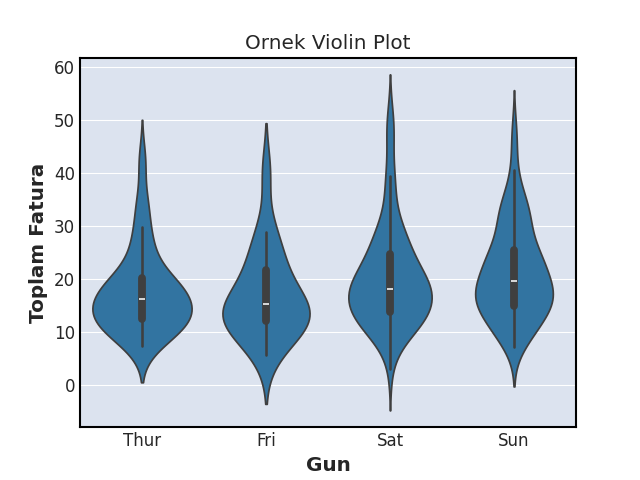
\includegraphics[width=0.7\textwidth]{images/violin_plot.png}
    \caption{Violin plot örneği.}
    \label{fig:enter-label}
\end{figure}

\newpage

\subsection{Box Plot}
Sayısal veri setlerinin dağılımını, merkezi eğilimini ve değişkenliğini görselleştirmek için kullanılan bir grafik türüdür. Veri setinin beş numaralı özeti (five number summary: minimum, birinci çeyrek, medyan, üçüncü çeyrek, maksimum) üzerine odaklanır. Gruplar arasındaki farklılıkları karşılaştırmak veya aykırı değerleri belirlemek için kullanılır. Kutunun alt sınırı birinci çeyrek (Q1), üst sınırı üçüncü çeyrek (Q3), ortadaki çizgi medyanı temsil eder. Kutunun uzunluğu verinin çeyrekler arası genişliğini (verinin yayılımını) gösterir. Aykırı değerler, alt veya üst sınırın dışında yer alan noktalar olarak gösterilir.

\begin{lstlisting}[language=Python]
import seaborn as sns
import matplotlib.pyplot as plt

tips = sns.load_dataset("tips")

sns.boxplot(x="day", y="total_bill", data=tips)
plt.title('Ornek Box Plot')
plt.xlabel('Gun')
plt.ylabel('Toplam Fatura')
plt.show()
\end{lstlisting}

\begin{figure}[h]
    \centering
    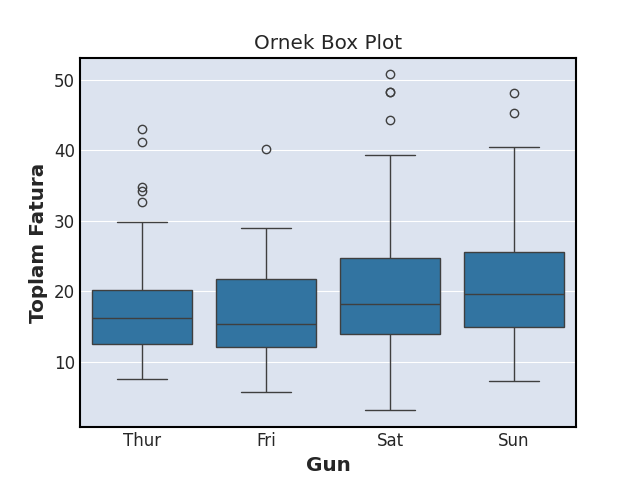
\includegraphics[width=0.7\textwidth]{images/box_plot.png}
    \caption{Box plot örneği.}
    \label{fig:enter-label}
\end{figure}

\newpage

\subsection{Stacked Area Chart}
Zamanla değişen kategorik verilerin toplamını veya oransal dağılımını görselleştirmek için kullanılır. Grafiğin üst kısmındaki toplam alan, tüm kategorilerin toplam değerini gösterir.

\begin{lstlisting}[language=Python]
import matplotlib.pyplot as plt

categories = ['Kategori 1', 'Kategori 2', 'Kategori 3']
values1 = [20, 30, 25]
values2 = [15, 25, 30]
values3 = [25, 20, 10]

plt.stackplot(categories, values1, values2, values3, labels=['Grup 1', 'Grup 2', 'Grup 3'])
plt.legend(loc='upper left')
plt.title('Ornek Stacked Area Chart')
plt.xlabel('Kategoriler')
plt.ylabel('Degerler')
plt.show()
\end{lstlisting}

\begin{figure}[h]
    \centering
    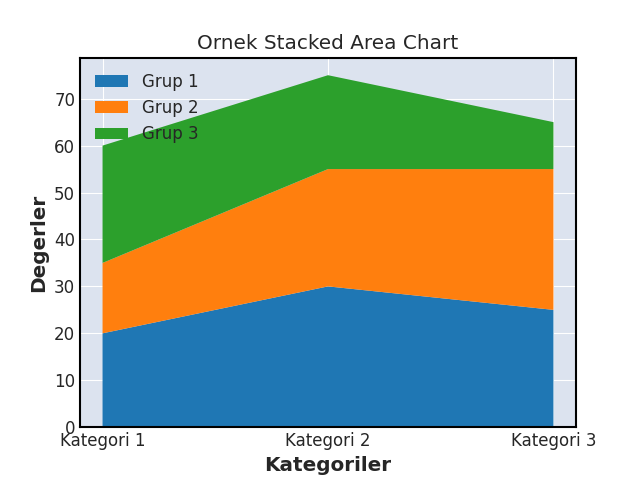
\includegraphics[width=0.7\textwidth]{images/stacked_area_chart.png}
    \caption{Stacked area chart örneği.}
    \label{fig:enter-label}
\end{figure}

\newpage

\subsection{Gantt Chart}
İş akışı sürecindeki görevlerin, aktivitelerin veya işlerin zaman içindeki ilerleyişini ve zamanlamasını temsil eder. Her bir çubuğun uzunluğu görevin ne kadar sürede tamamlanacağını gösterir. Çubukların başlangıç ve bitiş zamanları, ilgili görevlerin zamanlamasını gösterir.

\begin{lstlisting}[language=Python]
import plotly.figure_factory as ff

data = [
    dict(Task="Gorev 1", Start='2023-01-01', Finish='2023-01-31'),
    dict(Task="Gorev 2", Start='2023-02-01', Finish='2023-03-15'),
    dict(Task="Gorev 3", Start='2023-02-15', Finish='2023-04-10'),
]

fig = ff.create_gantt(data)
fig.show()
\end{lstlisting}

\begin{figure}[h]
    \centering
    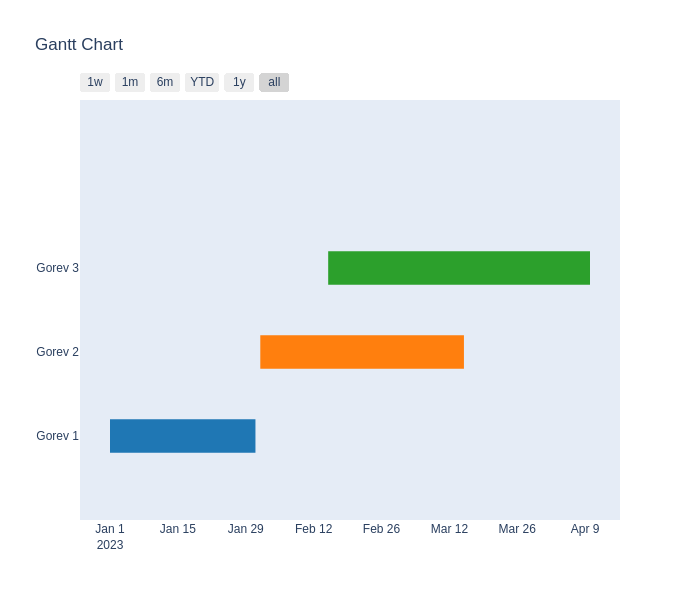
\includegraphics[width=0.7\textwidth]{images/gantt_chart.png}
    \caption{Gantt chart örneği.}
    \label{fig:enter-label}
\end{figure}

\newpage

\subsection{Dot Plot}
Her bir veri noktasını temsil etmek için noktalar kullanılır. Kategorik veya sayısal verilerin frekanslarını veya değerlerini görselleştirmek için kullanılır. Noktaların yoğun olduğu bölgeler, o değerin veri setinde daha sık veya yoğun olduğunu gösterir. Veri setinin dağılımını anlamak için kullanılır.

\begin{lstlisting}[language=Python]
import seaborn as sns
import matplotlib.pyplot as plt

data = [5, 7, 8, 7, 2, 17, 2, 9, 4, 11, 12, 9, 6]

sns.stripplot(data, jitter=True, marker='o', alpha=0.5)

plt.title('Ornek Dot Plot')
plt.xlabel('Degerler')
plt.show()
\end{lstlisting}

\begin{figure}[h]
    \centering
    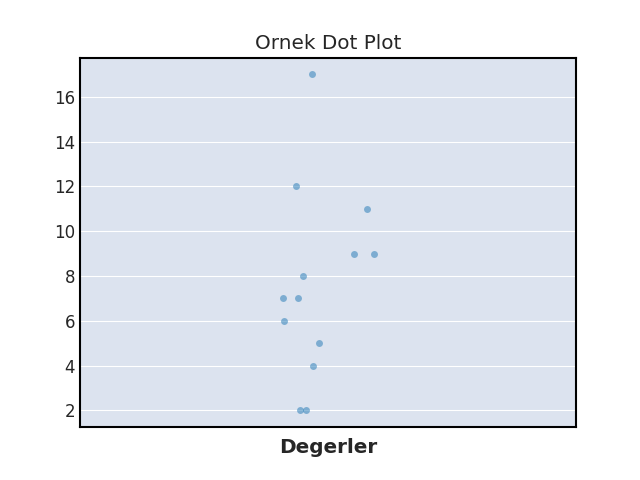
\includegraphics[width=0.7\textwidth]{images/dot_plot.png}
    \caption{Dot plot örneği.}
    \label{fig:enter-label}
\end{figure}

\newpage

\subsection{Scatter Plot}
İki sayısal değişken arasındaki ilişkiyi görselleştirmek için kullanılır. Veri noktalarının dağılımını, korelasyonu veya ilişkiyi görsel olarak göstermek için kullanılır. Eğer noktalar bir doğru veya belirli bir modele yakınsa, bu iki değişken arasında pozitif veya negatif bir korelasyon olduğunu gösterebilir. Eğer noktalar rastgele ve yayılmışsa, iki değişken arasında belirgin bir ilişki olmayabilir.

\begin{lstlisting}[language=Python]
import matplotlib.pyplot as plt

x = [5, 7, 8, 7, 2, 17, 2, 9, 4, 11, 12, 9, 6]
y = [99, 86, 87, 88, 111, 86, 103, 87, 94, 78, 77, 85, 86]

plt.scatter(x, y)

plt.title('Ornek Scatter Plot')
plt.xlabel('X Degeri')
plt.ylabel('Y Degeri')
plt.show()
\end{lstlisting}

\begin{figure}[h]
    \centering
    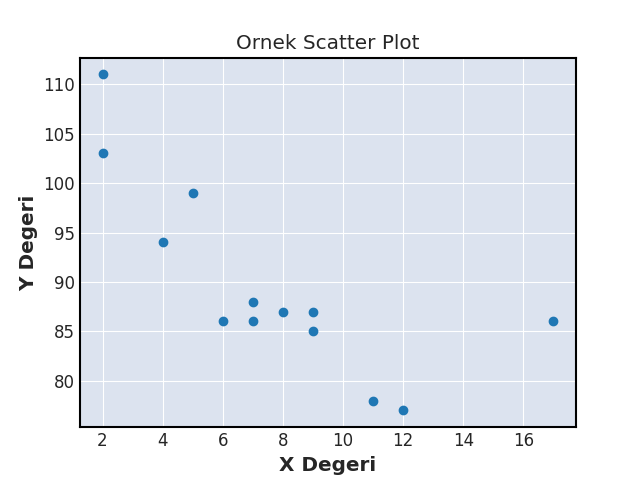
\includegraphics[width=0.7\textwidth]{images/scatter_plot.png}
    \caption{Scatter plot örneği.}
    \label{fig:enter-label}
\end{figure}

\newpage

\subsection{Histogram}
Bir veri setinin dağılımını göstermek için kullanılır. Özellikle sayısal verilerin frekans dağılımını incelemek için kullanılır. Veri setinin değerlerini belirli aralıklara böler ve her aralıktaki gözlem sayısını gösterir. Her bir sütun, belirli bir değer aralığındaki gözlem sayısını ifade eder.

\begin{lstlisting}[language=Python]
import matplotlib.pyplot as plt
import numpy as np

data = np.random.randn(1000)

plt.hist(data, bins=30, edgecolor='black')
plt.title('Ornek Histogram')
plt.xlabel('Degerler')
plt.ylabel('Frekans')
plt.show()
\end{lstlisting}

\begin{figure}[h]
    \centering
    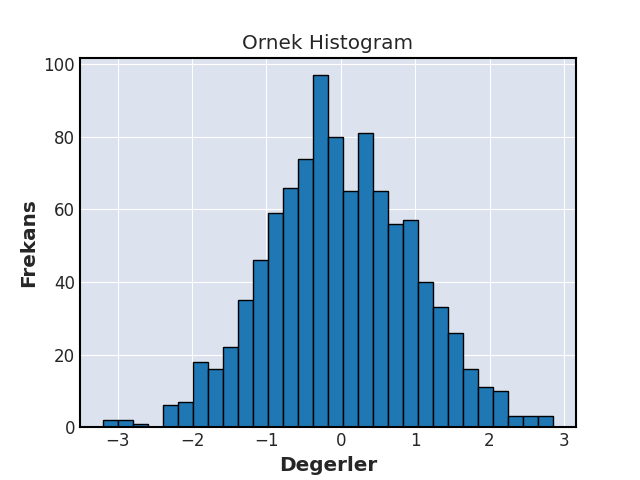
\includegraphics[width=0.7\textwidth]{images/histogram.png}
    \caption{Histogram örneği.}
    \label{fig:enter-label}
\end{figure}

\newpage

\subsection{Waterfall Chart}
Bir başlangıç noktasından başlayarak ardışık artışları veya azalışları görsel olarak temsil etmek için kullanılır. Her bir çubuk önceki değerin üzerine eklenir veya azalır ve toplam sonuca ulaşır. Pozitif değerler artışları, negatif değerler ise azalışları gösterir.

\begin{lstlisting}[language=Python]
import matplotlib.pyplot as plt

categories = ['Baslangic', 'Katki 1', 'Katki 2', 'Katki 3', 'Katki 4', 'Toplam']
values = [100, 50, 30, -20, -40, 120]

plt.bar(categories, values, color='b')
plt.title('Ornek Waterfall Chart')
plt.xlabel('Kategoriler')
plt.ylabel('Degerler')
plt.show()  
\end{lstlisting}

\begin{figure}[h]
    \centering
    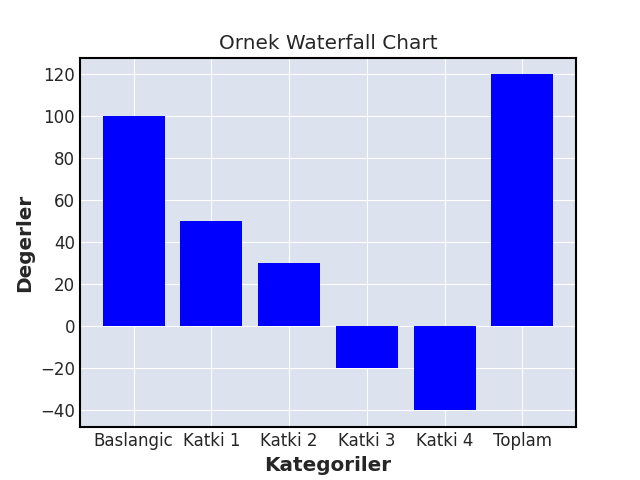
\includegraphics[width=0.7\textwidth]{images/waterfall_chart.png}
    \caption{Waterfall chart örneği.}
    \label{fig:enter-label}
\end{figure}

\newpage

\subsection{Convex Treemap}
Verileri hiyerarşik bir yapıda görselleştirmek için kullanılır.

\begin{lstlisting}[language=Python]
import matplotlib.pyplot as plt
import squarify

sizes = [25, 40, 15, 20]

squarify.plot(sizes, label=["Kategori 1", "Kategori 2", "Kategori 3", "Kategori 4"])
plt.axis('off')
plt.title('Treemap Ornegi')
plt.show()
\end{lstlisting}

\begin{figure}[h]
    \centering
    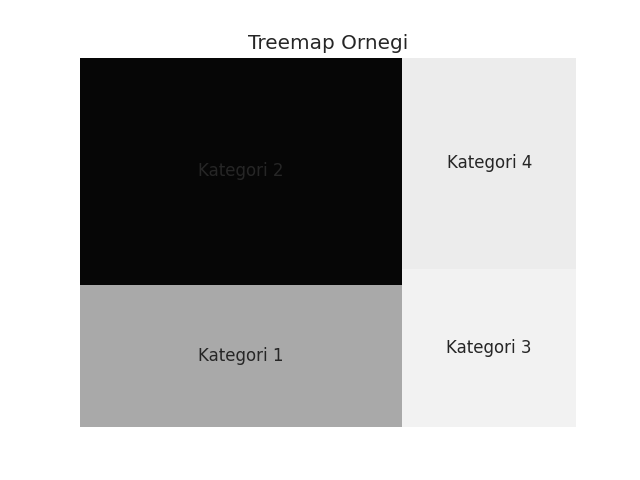
\includegraphics[width=0.7\textwidth]{images/convex_treemap.png}
    \caption{Convex treemap örneği.}
    \label{fig:enter-label}
\end{figure}

\newpage

\subsection{Bullet Graph}
Genellikle karşılaştırmalar yapmak için kullanılır. Özellikle hedeflerle gerçekleşen değerler arasındaki ilişkiyi göstermek için tercih edilir. İlgili değeri, hedefi ve gereken minimum-maksimum değer aralığını gösteren bir çizgi grafiği ve bir bar grafiğinden oluşur.

\begin{lstlisting}[language=Python]
import matplotlib.pyplot as plt
import numpy as np

categories = ['Kategori 1']
values = [80]
ranges = [(70, 90)]
targets = [85]

fig, ax = plt.subplots()
ax.set_title('Ornek Bullet Graph')

ax.set_ylim(0, 100)
ax.set_xlim(0, 1)

for i, val in enumerate(values):
    ax.barh(i, val, color='blue', height=0.3)

for i, (low, high) in enumerate(ranges):
    ax.plot([low, high], [i, i], color='black')

for i, target in enumerate(targets):
    ax.axvline(x=target, color='red', linewidth=2)

ax.set_yticks(np.arange(len(categories)))
ax.set_yticklabels(categories)

plt.show()
\end{lstlisting}

\begin{figure}[h]
    \centering
    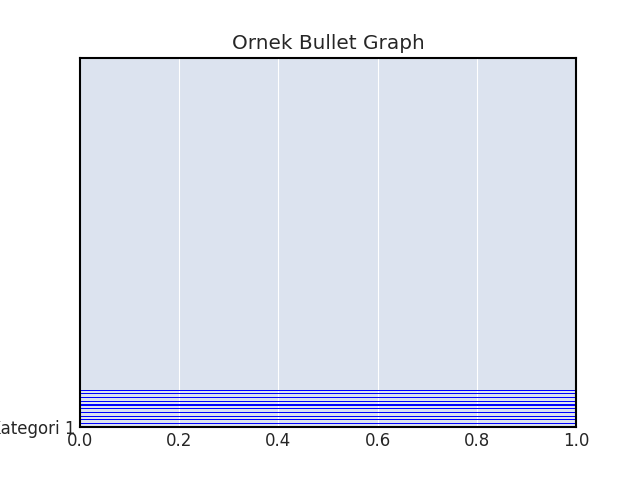
\includegraphics[width=0.4\textwidth]{images/bullet_graph.png}
    \caption{Bullet graph örneği.}
    \label{fig:enter-label}
\end{figure}

\newpage

\subsection{Pareto Chart}
Veri setindeki farklı kategorilerin katkısını ve önemini belirlemek için kullanılır. Pareto prensibi, belirli bir grubun toplamda katkısının genellikle tüm sonucun büyük bir kısmını oluşturduğunu öne sürer. Pareto chart, bu prensibi görselleştirir.

\begin{lstlisting}[language=Python]
import matplotlib.pyplot as plt

categories = ['Kategori A', 'Kategori B', 'Kategori C', 'Kategori D', 'Kategori E']
values = [50, 30, 20, 40, 60]

sorted_values, sorted_categories = zip(*sorted(zip(values, categories), reverse=True))

total = sum(values)

fig, ax1 = plt.subplots()

ax1.bar(sorted_categories, sorted_values, color='b')
ax1.set_ylabel('Degerler', color='b')
ax2 = ax1.twinx()
ax2.plot(sorted_categories, [100 * sum(sorted_values[:i+1])/total for i in range(len(sorted_values))], color='r', marker='o')
ax2.set_ylabel('Kumulatif Yuzde', color='r')
plt.title('Pareto Chart')
plt.xticks(rotation=45)
plt.show()
\end{lstlisting}

\begin{figure}[h]
    \centering
    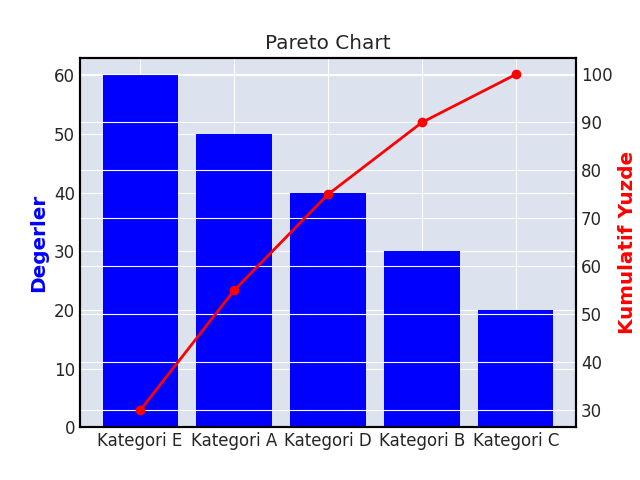
\includegraphics[width=0.7\textwidth]{images/pareto_chart.png}
    \caption{Pareto chart örneği.}
    \label{fig:enter-label}
\end{figure}

\newpage

\subsection{Candlestick Chart}
Finansal piyasalardaki fiyat hareketlerini görselleştirmek için kullanılır. Her bir mum, belirli bir zaman aralığındaki açılış, kapanış, en yüksek ve en düşük fiyatları gösterir. Her bir mumum gövdesi, açılış ve kapanış fiyatlarını, üst ve alt fitiller ise en yüksek ve en düşük fiyatları temsil eder. Mumların rengi kapanış fiyatlarının açılış fiyatından yüksek veya düşük olmasına göre değişir

\begin{lstlisting}[language=Python]
import mplfinance as mpf
import pandas as pd

data = {
    'Date': ['2023-01-01', '2023-01-02', '2023-01-03', '2023-01-04', '2023-01-05'],
    'Open': [100, 110, 105, 115, 120],
    'High': [120, 115, 125, 118, 130],
    'Low': [95, 105, 100, 110, 115],
    'Close': [115, 107, 122, 112, 125]
}

df = pd.DataFrame(data)
df['Date'] = pd.to_datetime(df['Date'])
df.set_index('Date', inplace=True)

mpf.plot(df, type='candle', style='yahoo', title='Ornek Candlestick Chart')
\end{lstlisting}

\begin{figure}[h]
    \centering
    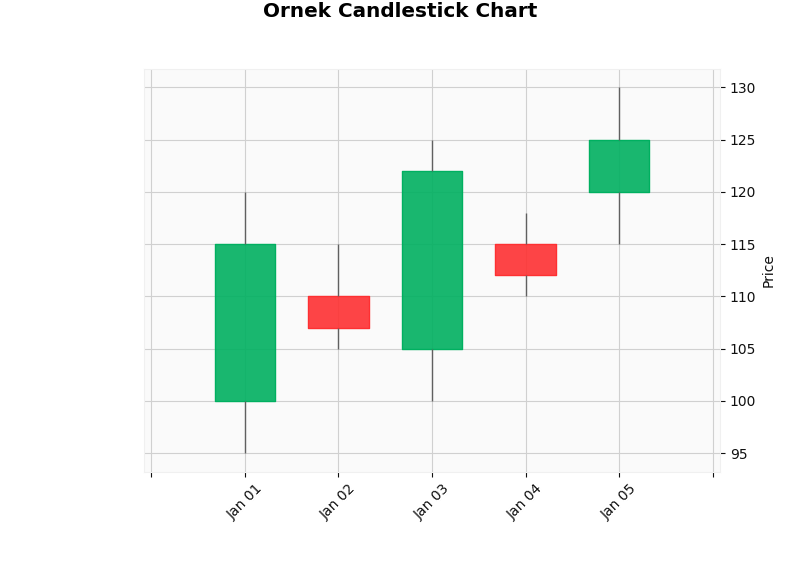
\includegraphics[width=0.7\textwidth]{images/candlestick_chart.png}
    \caption{Candlestick chart örneği.}
    \label{fig:enter-label}
\end{figure}

\newpage

\subsection{Contour Plot}
Üçüncü bir boyuttaki veri setlerini görselleştirmek için kullanılır. x ve y eksenlerindeki değerlerle ilişkilendirilmiş bir z-değeri ile temsil edilir. Bu grafik, eşit z değerlerinin eşit yükseklikte olduğu hatları gösterir. Böylece bir yüzeyin eşit yükseklikteki noktalarının bir haritasını sunar. Kontur çizgileri aynı z değerine sahip noktaları birleştirir. Çizgilerin yoğunlaştığı bölgelerde, yüzeyin o noktasında z değerlerinin daha yüksek veya düşük olduğu anlaşılır.

\begin{lstlisting}[language=Python]
import numpy as np
import matplotlib.pyplot as plt

x = np.linspace(-2, 2, 100)
y = np.linspace(-2, 2, 100)
X, Y = np.meshgrid(x, y)
Z = np.sin(np.sqrt(X**2 + Y**2))

plt.contour(X, Y, Z, levels=20)
plt.title('Contour Plot Ornegi')
plt.xlabel('X ekseni')
plt.ylabel('Y ekseni')
plt.colorbar(label='Z degerleri')
plt.show() 
\end{lstlisting}

\begin{figure}[h]
    \centering
    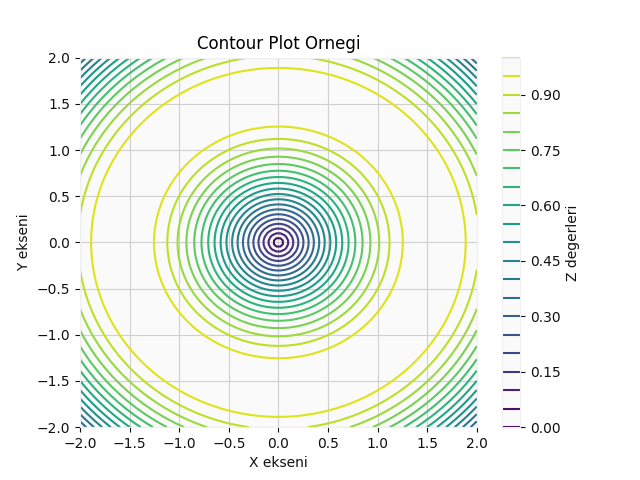
\includegraphics[width=0.7\textwidth]{images/contour_plot.png}
    \caption{Contour plot örneği.}
    \label{fig:enter-label}
\end{figure}

\newpage

\subsection{Kagi Chart}
Finansal piyasalarda fiyat hareketlerini temsil etmek için kullanılır. Zaman aralıklarındaki fiyat değişimlerini gösterirken, trendleri vurgulamak için kullanılır. Diğer finansal grafik türlerinden farklı olarak, zaman yerine fiyat değişimlerine dayalı olarak oluşturulur. Yüksek ve düşük fiyatlar arasındaki değişimler, trendin yönünü ve gücünü göstermek için belirli kurallara göre çizgi grafiklerle temsil edilir.

\begin{lstlisting}[language=Python]
import plotly.graph_objects as go

dates = ['2023-01-01', '2023-01-02', '2023-01-03', '2023-01-04', '2023-01-05']
prices = [100, 110, 105, 115, 120]

fig = go.Figure(go.Scatter(x=dates, y=prices, mode='lines', line=dict(width=1)))

fig.update_layout(
    title='Ornek Kagi Chart',
    xaxis=dict(title='Tarih'),
    yaxis=dict(title='Fiyat'),
)

fig.show()
\end{lstlisting}

\begin{figure}[h]
    \centering
    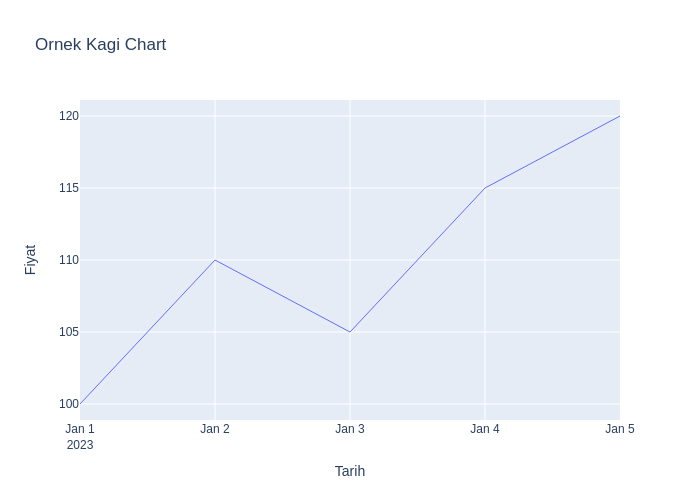
\includegraphics[width=0.7\textwidth]{images/kagi_chart.png}
    \caption{Kagi chart örneği.}
    \label{fig:enter-label}
\end{figure}

\newpage

\subsection{RainCloud Plot}
Box Plot, Strip Plot ve KDE Plot'u tek bir grafikte gösterir.

\begin{lstlisting}[language=Python]
import ptitprince as pt

pt.RainCloud(df, x="money", y="item")
\end{lstlisting}

\newpage

\subsection{Span Chart}
Verilerin zaman göre değişimini gösterme için kullanılır. Bir zaman aralığındaki değerlerin üst ve alt sınırlarını belirtirken, ortalamasını da gösterir.

\begin{lstlisting}[language=Python]
import matplotlib.pyplot as plt
import numpy as np

np.random.seed(42)
time = np.arange(1, 21)
values = np.random.normal(0, 1, 20)
mean = np.mean(values)
std_dev = np.std(values)

plt.plot(time, values, marker='o', linestyle='-', color='blue', label='Degerler')
plt.axhline(mean, color='green', linestyle='--', label='Ortalama')
plt.fill_between(time, mean - std_dev, mean + std_dev, color='yellow', alpha=0.3, label='Standart Sapma')
plt.title('Ornek Span Chart')
plt.xlabel('Zaman')
plt.ylabel('Degerler')
plt.legend()
plt.grid(True)
plt.show()
\end{lstlisting}

\begin{figure}[h]
    \centering
    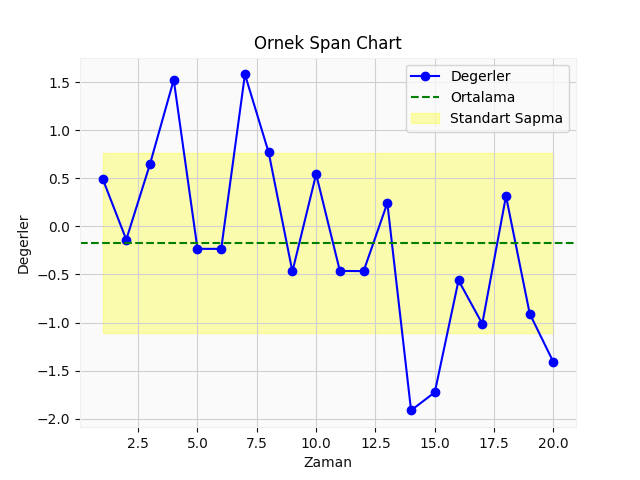
\includegraphics[width=0.7\textwidth]{images/span_chart.png}
    \caption{Span chart örneği.}
    \label{fig:enter-label}
\end{figure}

\newpage

\subsection{Spline Graph}
Eğri veya kavisli hatlarla verileri görselleştirir. Veri noktaları arasında yumuşak bir geçiş oluşturarak veri setindeki genel trendi gösterir.

\begin{lstlisting}[language=Python]
import matplotlib.pyplot as plt
import numpy as np

x = np.linspace(0, 10, 100)
y = np.sin(x)

plt.plot(x, y, label='Veri', color='blue')
plt.plot(x, y, label='Spline', color='red', linestyle='-', marker='o')
plt.title('Ornek Spline Chart')
plt.xlabel('X ekseni')
plt.ylabel('Y ekseni')
plt.legend()
plt.grid(True)
plt.show()
\end{lstlisting}

\begin{figure}[h]
    \centering
    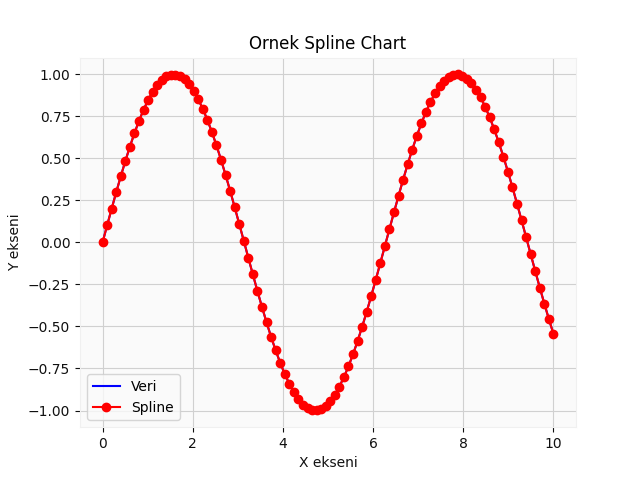
\includegraphics[width=0.7\textwidth]{images/spline_graph.png}
    \caption{spline graph örneği.}
    \label{fig:enter-label}
\end{figure}

\newpage

\subsection{Slope Chart}
İki farklı zaman veya kategori noktası arasındaki bağlantıları ve değişiklikleri göstermek için kullanılır.

\begin{lstlisting}[language=Python]
import matplotlib.pyplot as plt

categories = ['2019', '2020', '2021']
values_A = [20, 35, 50]
values_B = [30, 45, 55]

plt.plot(categories, values_A, marker='o', label='Kategori A')
plt.plot(categories, values_B, marker='o', label='Kategori B')

for i in range(len(categories)):
    plt.plot([categories[i], categories[i]], [values_A[i], values_B[i]], linestyle='--', color='gray')

plt.title('Ornek Slope Chart')
plt.xlabel('Zaman')
plt.ylabel('Degerler')
plt.legend()
plt.grid(True)
plt.show()
\end{lstlisting}

\begin{figure}[h]
    \centering
    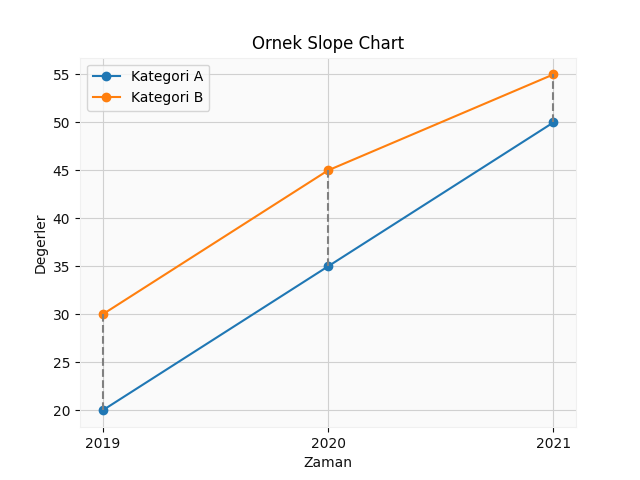
\includegraphics[width=0.7\textwidth]{images/slope_chart.png}
    \caption{Slope chart örneği.}
    \label{fig:enter-label}
\end{figure}

\newpage

\subsection{Butterfly Chart}
Bir ana kategorinin alt kategorilerinin performansını gösterirken her alt kategorinin iki yönlü (olumlu ve olumsuz) etkilerini vurgular.

\begin{lstlisting}[language=Python]
import matplotlib.pyplot as plt

categories = ['Kategori A', 'Kategori B', 'Kategori C', 'Kategori D']
positive_values = [10, 15, 12, 18]
negative_values = [-8, -10, -5, -12]

fig, ax = plt.subplots()
ax.barh(categories, positive_values, color='green', label='Pozitif')
ax.barh(categories, negative_values, color='red', label='Negatif')
ax.axvline(x=0, color='black', linewidth=0.8)
plt.title('Ornek Butterfly Chart')
plt.xlabel('Degerler')
plt.legend()
plt.grid(axis='x')
plt.show()
\end{lstlisting}

\begin{figure}[h]
    \centering
    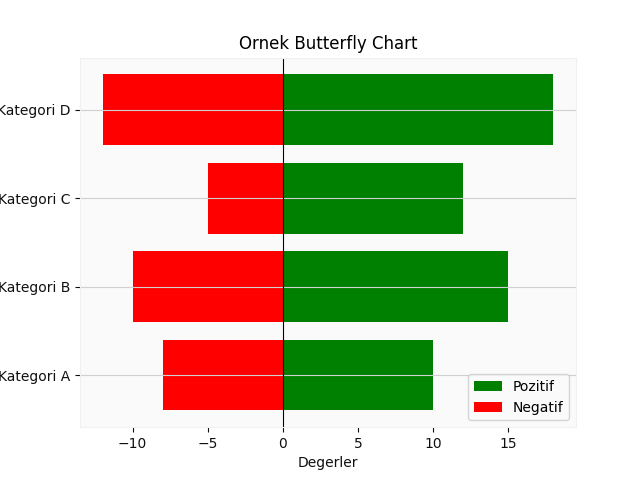
\includegraphics[width=0.7\textwidth]{images/butterfly_chart.png}
    \caption{Butterfly Chart örneği.}
    \label{fig:enter-label}
\end{figure}

\newpage

\subsection{Renko Chart}
Fiyat hareketlerini görselleştirmek için kullanılır. Zamanı dikkate almaz ve sadece fiyat hareketlerine dayanarak bloklar oluşturur. Her bir blok, fiyatın belirli bir miktar veya eşik değerinde değiştiği durumları temsil eder.

\begin{lstlisting}[language=Python]
import pandas as pd
import mplfinance as mpf

data = {
    'Date': ['2023-01-01', '2023-01-02', '2023-01-03', '2023-01-04', '2023-01-05'],
    'Open': [100, 110, 105, 115, 120],
    'High': [120, 115, 125, 118, 130],
    'Low': [95, 105, 100, 110, 115],
    'Close': [115, 107, 122, 112, 125]
}

df = pd.DataFrame(data)
df['Date'] = pd.to_datetime(df['Date'])
df.set_index('Date', inplace=True)

mpf.plot(df, type='renko', title='Ornek Renko Chart')
\end{lstlisting}

\newpage

\subsection{Marimekko Chart}
Kategorik verilerin hem yüzde dağılımlarını hem de toplam büyüklüklerini göstermek için kullanılır. Blokların genişliği temsil edilen kategorilerin yüzde dağılımlarını, blokların yüksekliği toplam büyüklükleri gösterir.

\begin{lstlisting}[language=Python]
import plotly.graph_objects as go

categories = ['Kategori A', 'Kategori B', 'Kategori C', 'Kategori D']
values = [25, 40, 15, 20]
totals = [100, 150, 80, 120]

percentages = [val / total * 100 for val, total in zip(values, totals)]

fig = go.Figure(go.Bar(
    x=percentages,
    y=categories,
    orientation='h',
    text=values,
    textposition='inside',
    texttemplate='%{text}',
    marker=dict(color='skyblue'),
    width=[val / total for val, total in zip(values, totals)]
))

fig.update_layout(
    title='Ornek Marimekko Chart',
    xaxis=dict(title='Yuzde (%)'),
    yaxis=dict(title='Kategoriler'),
    bargap=0.2 
)

fig.show()
\end{lstlisting}

\begin{figure}[h]
    \centering
    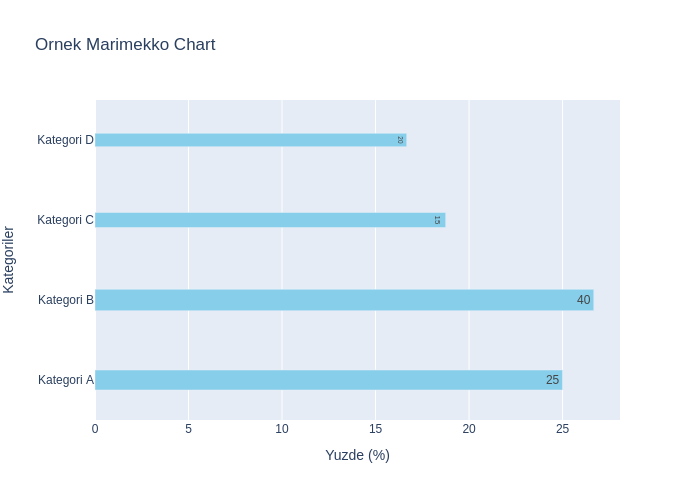
\includegraphics[width=0.4\textwidth]{images/marimekko_chart.png}
    \caption{Marimekko Chart örneği.}
    \label{fig:enter-label}
\end{figure}

\newpage

\subsection{3D Scatter Plot}
Üç boyutlu uzayda verilerin dağılımlarını görselleştirir. Üç farklı değişkenin birbirine göre ilişkisini göstermek için kullanılır. Her bir nokta, üç farklı değişkenin belirli bir kombinasyonunu temsil eder.

\begin{lstlisting}[language=Python]
import matplotlib.pyplot as plt
from mpl_toolkits.mplot3d import Axes3D
import numpy as np

np.random.seed(0)
x = np.random.rand(100)
y = np.random.rand(100)
z = np.random.rand(100)

fig = plt.figure()
ax = fig.add_subplot(111, projection='3d')
ax.scatter(x, y, z, c='blue', marker='o')
ax.set_xlabel('X ekseni')
ax.set_ylabel('Y ekseni')
ax.set_zlabel('Z ekseni')
plt.title('Ornek 3D Scatter Plot')
plt.show()
\end{lstlisting}

\begin{figure}[h]
    \centering
    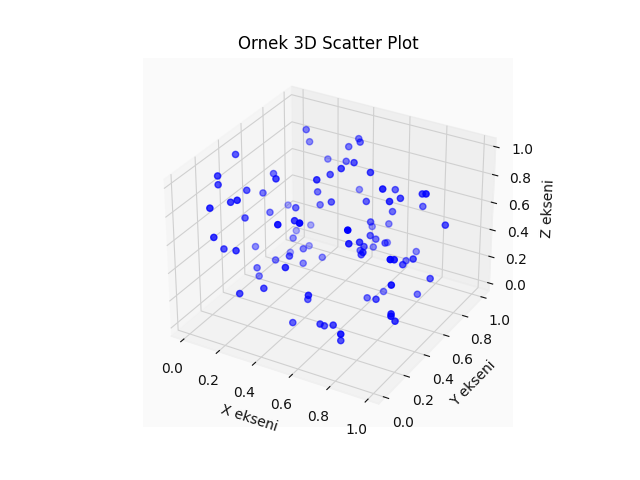
\includegraphics[width=0.7\textwidth]{images/3d_scatter_plot.png}
    \caption{3D scatter plot örneği.}
    \label{fig:enter-label}
\end{figure}

\newpage

\subsection{Fan Chart}
Gelecekteki belirsizliği ve değişkenliği göstermek için kullanılır. Tahminlerin olası farklı senaryolarını göstermek için kullanılır. Zaman serileri üzerinde kullanılır ve belirli bir zaman aralığındaki muhtemel değerlerin aralığını vurgular. Çizgi grafiği ile gösterilen belirsizlik aralığı, gelecekteki muhtemel değerlerin aralığını vurgular.

\begin{lstlisting}[language=Python]
import matplotlib.pyplot as plt
import numpy as np

np.random.seed(0)
time = np.arange(0, 10, 1)
values = np.random.normal(0, 1, 10)
uncertainty = 0.2

plt.plot(time, values, color='blue', label='Degerler')
plt.fill_between(time, values - uncertainty, values + uncertainty, color='blue', alpha=0.2, label='Belirsizlik Araligi')
plt.title('Ornek Fan Chart')
plt.xlabel('Zaman')
plt.ylabel('Degerler')
plt.legend()
plt.grid(True)
plt.show()
\end{lstlisting}

\begin{figure}[h]
    \centering
    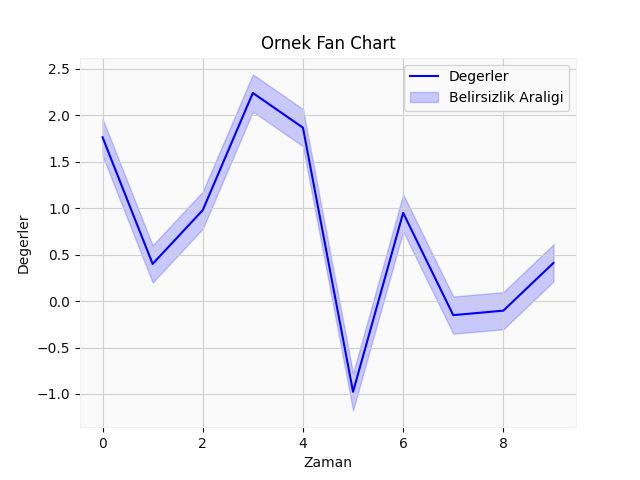
\includegraphics[width=0.7\textwidth]{images/fan_chart.png}
    \caption{Fan chart örneği.}
    \label{fig:enter-label}
\end{figure}

\newpage

\subsection{Dendrogram}
Hiyerarşik kümeleme analizlerinde kullanılır. Benzer özelliklere sahip veri noktalarını veya gözlemleri gruplar. Yatay çizgi ne kadar uzunsa, o gözlemler arasındaki benzerlik o kadar düşüktür. Veri setindeki farklı düzeylerdeki grupların birbiriyle nasıl ilişkilendiğini veya nasıl birbirinden ayrıldığını gösterir.

\begin{lstlisting}[language=Python]
from scipy.cluster import hierarchy
import matplotlib.pyplot as plt
import numpy as np

np.random.seed(123)
data = np.random.rand(10, 2)

dendrogram = hierarchy.linkage(data, method='single')

plt.figure(figsize=(8, 5))
plt.title('Ornek Dendrogram')
plt.xlabel('Gozlem Birimleri')
plt.ylabel('Uzaklik')
hierarchy.dendrogram(dendrogram)
plt.show()
\end{lstlisting}

\begin{figure}[h]
    \centering
    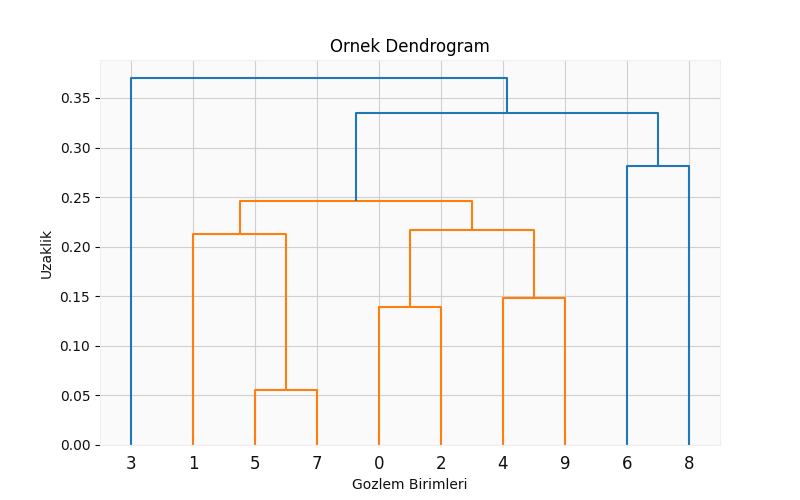
\includegraphics[width=0.7\textwidth]{images/dendrogram.png}
    \caption{Dendrogram örneği.}
    \label{fig:enter-label}
\end{figure}

\newpage

\subsection{Jitter Plot}
Veri noktalarının yoğun olduğu alanlarda, özellikle kategorik verilerle çalışırken noktaların üst üste gelmesini önlemek ve dağılımı daha iyi görselleştirmek için kullanılır. Her bir nokta, kategorik bir değişkenin değeriyle ilişkilendirilen sürekli bir değişkenin değerini temsil eder.

\begin{lstlisting}[language=Python]
import seaborn as sns
import matplotlib.pyplot as plt
import pandas as pd
import numpy as np

np.random.seed(0)
categories = ['A', 'B', 'C', 'D']
values = np.random.rand(100)
categories = np.random.choice(categories, 100)

data = pd.DataFrame({'Category': categories, 'Value': values})

plt.figure(figsize=(8, 6))
sns.stripplot(x='Category', y='Value', data=data, jitter=True, alpha=0.7)
plt.title('Ornek Jitter Plot')
plt.xlabel('Kategoriler')
plt.ylabel('Degerler')
plt.show()
\end{lstlisting}

\begin{figure}[h]
    \centering
    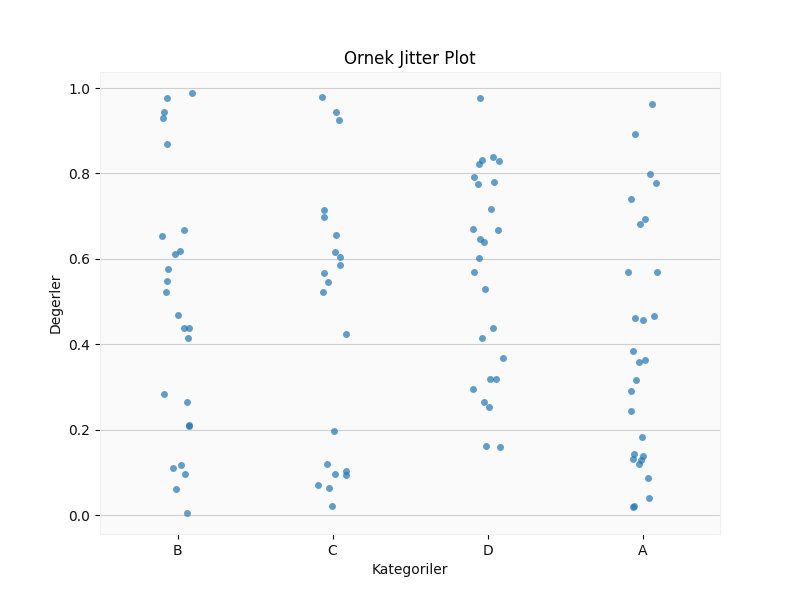
\includegraphics[width=0.7\textwidth]{images/jitter_plot.png}
    \caption{Jitter plot örneği.}
    \label{fig:enter-label}
\end{figure}

\newpage

\subsection{Strip Plot}
Kategorik bir değerle ilişkilendirilmiş sürekli bir değişkenin dağılımını göstermek için kullanılır. Her bir veri noktasını yatay bir eksen boyunca düzenler ve kategorik değişkenin değerlerine göre dağılımı görselleştirir.

\begin{lstlisting}[language=Python]
import seaborn as sns
import matplotlib.pyplot as plt
import pandas as pd
import numpy as np

np.random.seed(0)
categories = ['A', 'B', 'C', 'D']
values = np.random.rand(100)
categories = np.random.choice(categories, 100)

data = pd.DataFrame({'Category': categories, 'Value': values})

plt.figure(figsize=(8, 6))
sns.stripplot(x='Category', y='Value', data=data, alpha=0.7)
plt.title('Ornek Strip Plot')
plt.xlabel('Kategoriler')
plt.ylabel('Degerler')
plt.show()
\end{lstlisting}

\newpage

\subsection{QQ Plot}
Bir veri setinin normal dağılımından gelip gelmediğini belirmek için kantilleri kullanan grafik türüdür. Öncelikle veriler küçükten büyüğe doğru sıralanır. Daha sonra sıralanan veriler ile standart normal dağılımın tablo değerleri koordinat sisteminde gösterilir. Eğer veriler doğrusal bir çizgi üzerinde yayılım gösteriyorsa verilerin normal dağılıma sahip olduğu söylenir.

\begin{lstlisting}[language=Python]
import numpy as np
import matplotlib.pyplot as plt
import statsmodels.api as sm

# Ornek veri olusturma
np.random.seed(42)
normal_data = np.random.normal(loc=0, scale=1, size=1000)

# QQ Plot olusturma
sm.qqplot(normal_data, line ='45')
plt.title('QQ Plot - Normal Dagilim')
plt.savefig('qq_plot')
plt.show()
\end{lstlisting}

\begin{figure}[h]
    \centering
    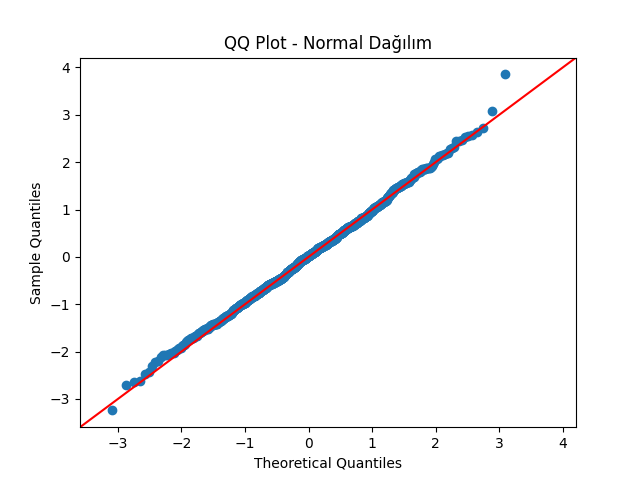
\includegraphics[width=0.6\textwidth]{images/qq_plot.png}
    \caption{QQ Plot örneği.}
    \label{fig:enter-label}
\end{figure}

\newpage

\subsection{KS Plot}
KS (Kolmogorov-Smirnov) plot, veri setinin belirli bir teorik dağılıma uyumunu görselleştirmek için kullanılan bir grafik analiz aracıdır. KS plot, kümülatif dağılım fonksiyonunun (CDF) gerçek ve teorik dağılımlar arasındaki farkı gösterir. Bu fark, genellikle bir çizgi veya çizgi grafiği şeklinde gösterilir. KS plot, ayrıca "empirik dağılım fonksiyonu" (ECDF) ile "teorik dağılım fonksiyonu" arasındaki farkı da görselleştirir. ECDF, gözlemlenen veri setinin dağılımını temsil ederken, teorik dağılım fonksiyonu ise belirli bir teorik dağılımın beklenen dağılımını temsil eder. KS plot'un eğrisi, gerçek ve teorik CDF'ler arasındaki farkı gösterir. Eğer bu fark beklenenin dışındaysa, yani eğri belirli bir mesafeden uzaklaşıyorsa, bu veri setinin teorik dağılıma iyi uyum sağlamadığı anlamına gelir. Eğri, iki CDF arasındaki farkın büyüklüğüne göre değerlendirilebilir.

\begin{lstlisting}[language=Python]
import numpy as np
import matplotlib.pyplot as plt
import statsmodels.api as sm

# Ornek veri seti olusturma
np.random.seed(42)
normal_data = np.random.normal(loc=0, scale=1, size=1000)

# Teorik dagilim
theoretical_distribution = np.random.normal(loc=0, scale=1, size=1000)

# KS plot olusturma
sm.qqplot_2samples(normal_data, theoretical_distribution, line ='45')
plt.title('KS Plot - Normal Dagilim')
plt.savefig('ks_plot')
plt.show()
\end{lstlisting}

\begin{figure}[h]
    \centering
    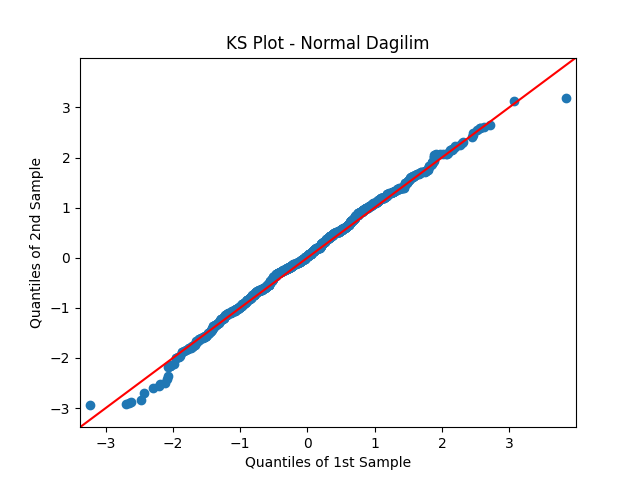
\includegraphics[width=0.5\textwidth]{images/ks_plot.png}
    \caption{KS Plot örneği.}
    \label{fig:enter-label}
\end{figure}

\newpage 